{$H_0:\theta=0$}
Assume hypothesis
$H_0:\theta=0$ is true.
\begin{enumerate}
\item Given X is symmetric around zero.
 \begin{align}
  f_X(x)&=f_X(-x)\\
  \int_{0}^{\infty}f_X(x)dx&=\int_{0}^{\infty}f_X(-x)dx
  \label{june/2012/112/int}
\end{align}
\begin{enumerate}
\item Solving LHS of $\eqref{june/2012/112/int}$
\begin{align}
    \int_{0}^{\infty}f_X(x)dx=\pr{X\geq0}
\end{align}
\item Solving RHS of $\eqref{june/2012/112/int}$
\begin{align}
    \int_{0}^{\infty}f_X(-x)dx
\end{align}
Changing $-x \rightarrow x$ we get 
\begin{align}
  \int_{0}^{\infty}f_X(-x)dx&=\int_{-\infty}^{0}f_X(x)dx\label{june/2012/112/rhs}\\
  &=\pr{X\leq0}
\end{align}
\end{enumerate}
but
\begin{align}
  \int_{-\infty}^{0}f_X(x)dx+\int_{0}^{\infty}f_X(x)dx=1
  \label{june/2012/112/pr}
\end{align}
from $\eqref{june/2012/112/int}$ , $\eqref{june/2012/112/rhs}$ and $\eqref{june/2012/112/pr}$
\begin{align}
\int_{-\infty}^{0}f_X(x)dx=\int_{0}^{\infty}f_X(x)dx=\frac{1}{2}
\end{align}
\begin{align}
    \implies \pr{X\leq 0}=\pr{X\geq0}=\frac{1}{2}
    \label{june/2012/112/sym}
\end{align}
\item Let Y be a random variable such that
\begin{align}
    Y=sign(X)
\end{align}
\begin{align}
    Y=
    \begin{cases}
     1 & X>0\\
    -1 & X<0
    \end{cases}
    \label{june/2012/112/t}
\end{align}
From $\eqref{june/2012/112/sym}$ and $\eqref{june/2012/112/t}$
we have
\begin{align}
   \pr{Y=-1}=\pr{Y=1}=\frac{1}{2} 
\end{align}
So $Y=sign(X)$ is also symmetric around zero.
% \begin{figure}[!ht]
% \centering
% 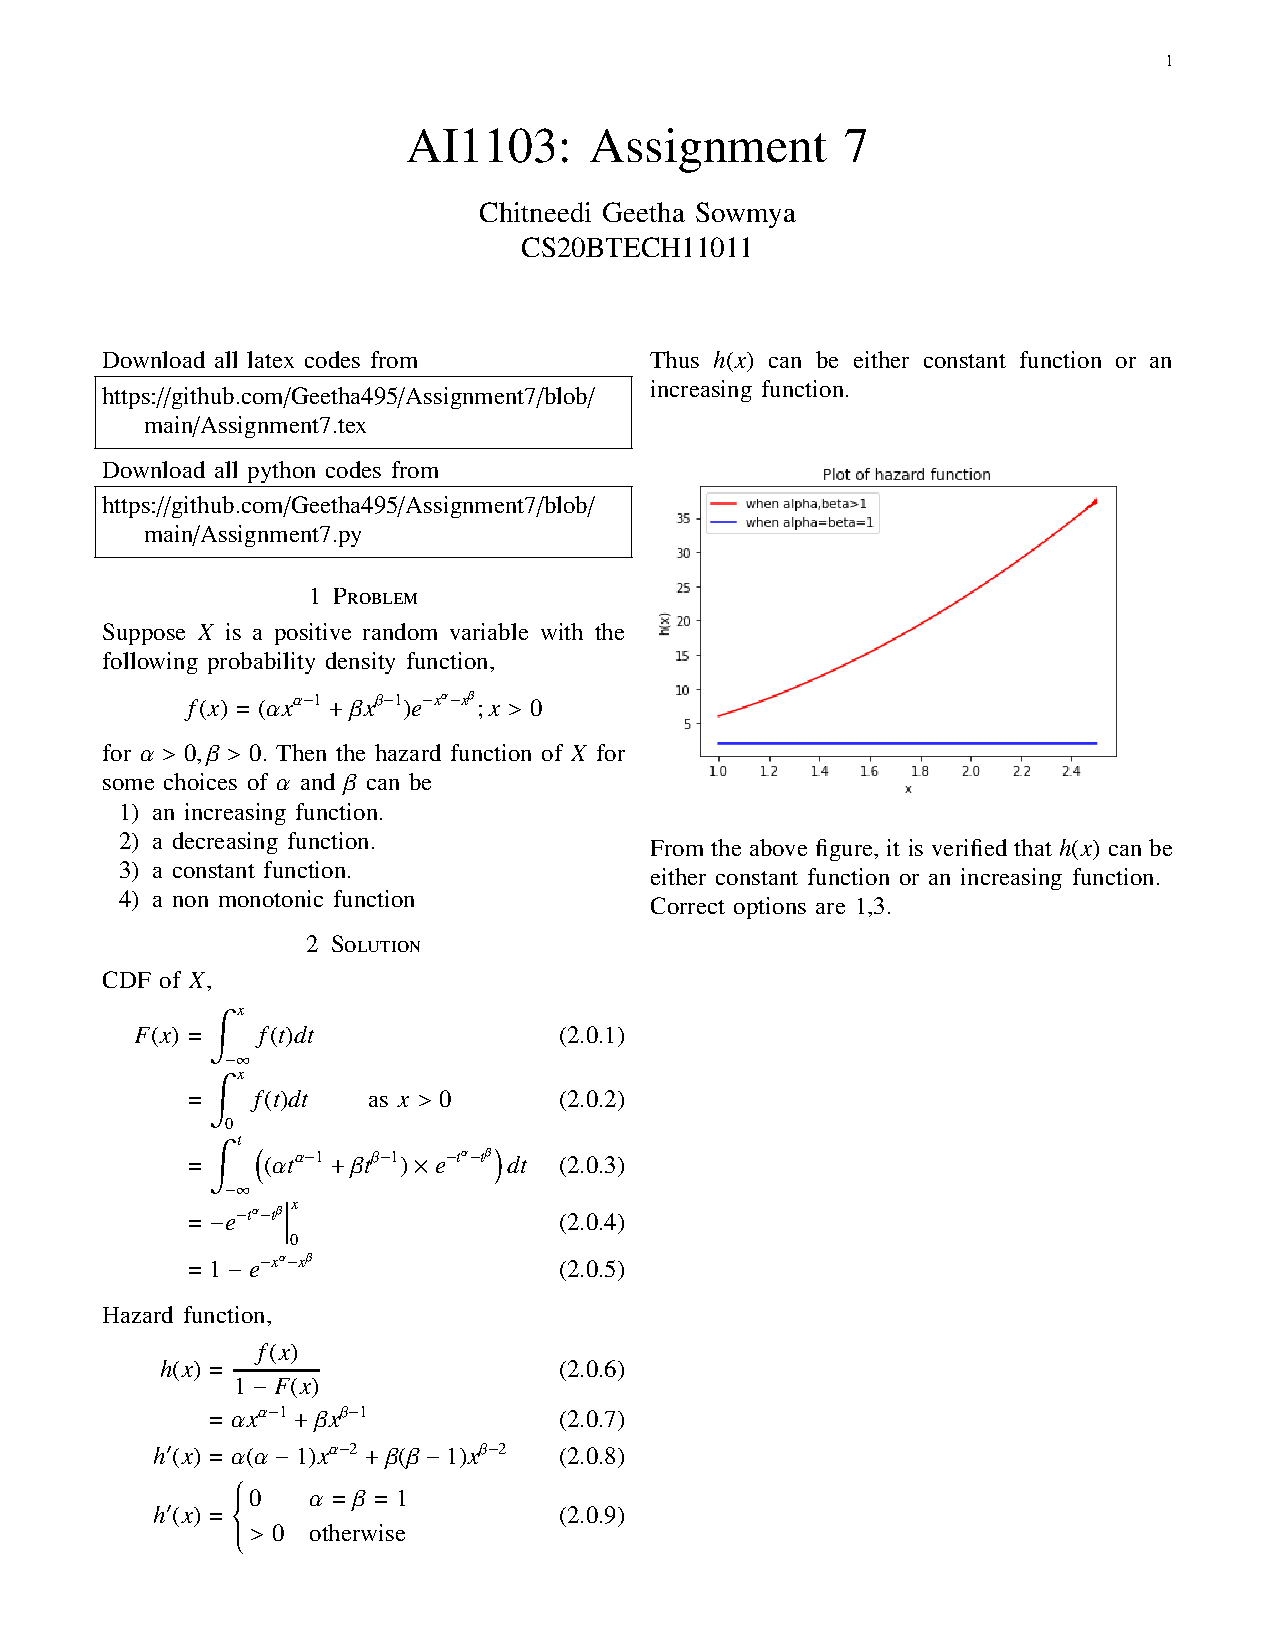
\includegraphics[width=\columnwidth]{Assignment7.png}
% \caption{pdf of $ Y=sign(X)$}
% \label{june/2012/112/pdf}
% \end{figure}
\begin{align}
   \implies \mu_y = 0 
\end{align}
and variance is
\begin{align}
    \sigma_y^2 &= (-1)^2\brak{\frac{1}{2}}+(1)^2\brak{\frac{1}{2}}\\
    &=1
\end{align}
\item Given
\begin{align}
    S_n&=\sum_{i=1}^{n} sign(X_i)\\
    S_n(\theta=0)&=\sum_{i=1}^{n} Y_i
\end{align}
From central limit theorem 
\begin{align}
    Z&=\lim_{n\to\infty}\sqrt{n}\brak{\frac{\frac{S_n}{n}-\mu_y}{\sigma_y}}\\
    &=\lim_{n\to\infty}\sqrt{n}\brak{\frac{S_n}{n}}\\
    &=\lim_{n\to\infty}\brak{\frac{S_n}{\sqrt{n}}}
    \label{june/2012/112/clt}
\end{align}
where Z is a standard normal variable N(0,1).
\begin{enumerate}
    \item Given
\begin{align}
    \alpha = P\cbrak{Z>z_\alpha}\label{june/2012/112/uff}
\end{align}
So from $\eqref{june/2012/112/clt}$ and $\eqref{june/2012/112/uff}$
\begin{align}
\lim_{n\to\infty}P\cbrak{\frac{S_n}{\sqrt{n}}>z_\alpha}&=
\alpha\\
\implies \lim_{n\to\infty}P\cbrak{S_n>\sqrt{n}z_\alpha}&=
\alpha
\end{align}
\end{enumerate}
\end{enumerate}
{$H_1:\theta >0$ is true}
\begin{enumerate}
    \item Given X is symmetric around $\theta>0$.Let us assume $\theta=\theta_0>0$.
    \begin{align}
        f_X(\theta_0-x)&=f_X(\theta_0+x)\\
        \int_{\theta_0}^{\infty} f_X(\theta_0-x)dx&=
        \int_{\theta_0}^{\infty} f_X(\theta_0+x)dx
        \label{june/2012/112/s}
    \end{align}
    \begin{enumerate}
        \item Solving LHS of $\eqref{june/2012/112/s}$.Changinng $(\theta_0-x) \rightarrow t$
        \begin{align}
           \int_{\theta_0}^{\infty} f_X(\theta_0-x)dx&=
           \int_{-\infty}^{0}f_X(t) dt\\
           &=\pr{X\leq0}\label{june/2012/112/temp}
        \end{align}
        \item Solving RHS of $\eqref{june/2012/112/s}$.Changing $(\theta_0+x) \rightarrow t$
        \begin{align}
           \int_{\theta_0}^{\infty} f_X(\theta_0+x)dx&=
           \int_{2\theta_0}^{\infty} f_X(t)dt\\
          &= \int_{0}^{\infty} f_X(t)dt-\int_{0}^{2\theta_0} f_X(t)dt\\
          &=\pr{X\geq0}-k\label{june/2012/112/u}
        \end{align}
        where
        \begin{align}
           k=\int_{0}^{2\theta_0} f_X(t)dt>0 
        \end{align}
    \end{enumerate}
    From $\eqref{june/2012/112/s}$,$\eqref{june/2012/112/t}$ and $\eqref{june/2012/112/u}$
    \begin{align}
        \pr{X\geq0}>\pr{X\leq0}
    \end{align}
    \item So
    \begin{align}
        \pr{Y=1}>\pr{Y=-1}
    \end{align}
    Therefore,if we perform the experiment and find the value of $\brak{\frac{S_n}{\sqrt{n}}}$,it is most likely to occur on the right side of the distribution of 
$\brak{\frac{S_n}{\sqrt{n}}}$.In $\eqref{june/2012/112/clt}$ it is shown that distrubution of the random variable $\brak{\frac{S_n}{\sqrt{n}}}$
 is $N(0,1)$ when n is very large.So
\begin{align}
    \lim_{n\to\infty}P\cbrak{\frac{S_n}{\sqrt{n}}>Z_\alpha}=1
\end{align}
\end{enumerate}